%Template by Mark Jervelund - 2015 - mjerv15@student.sdu.dk

\documentclass[a4paper,10pt,titlepage]{report}

\usepackage[utf8]{inputenc}
\usepackage[T1]{fontenc}
\usepackage[english]{babel}
\usepackage{amssymb}
\usepackage{amsmath}
\usepackage{amsthm}
\usepackage{graphicx}
\usepackage{fancyhdr}
\usepackage{lastpage}
\usepackage{pgfplots}
\usepackage{listings}
\usepackage{algorithm}
\usepackage{algpseudocode}
\usepackage{wrapfig}
\usepackage[document]{ragged2e}
\usepackage[margin=1in]{geometry}
\usepackage{enumitem}
\usepackage{color}
\usepackage{datenumber}
\usepackage{venndiagram}
\usepackage{chngcntr}
\setdatetoday
\addtocounter{datenumber}{0} %date for dilierry standard is today
\setdatebynumber{\thedatenumber}
\date{}
\setcounter{secnumdepth}{0}
\pagestyle{fancy}
\fancyhf{}


%lstlisting ting:
\definecolor{dkgreen}{rgb}{0,0.45,0}
\definecolor{gray}{rgb}{0.5,0.5,0.5}
\definecolor{mauve}{rgb}{0.30,0,0.30}
\lstset{frame=tb,
  language=C++,
  aboveskip=3mm,
  belowskip=3mm,
  showstringspaces=false,
  columns=flexible,
  basicstyle={\small\ttfamily},
  numbers=left,
  numberstyle=\footnotesize,
  keywordstyle=\color{dkgreen}\bfseries,
  commentstyle=\color{dkgreen},
  stringstyle=\color{mauve},
  frame=single,
  breaklines=true,
  breakatwhitespace=false
  tabsize=1
}
\renewcommand{\lstlistingname}{Code}

\newcommand{\Z}{\mathbb{Z}}
\lhead{Parallel Computinge (DM818))}
\rhead{Mark Jervelund (Mjerv15)}
\rfoot{Page  \thepage \, of \pageref{LastPage}}
\counterwithin*{equation}{section}

\begin{document}
\begin{titlepage}
\centering
    \vspace*{9\baselineskip}
    \huge
    \bfseries
    2. Mandatory Assignment \\
    \normalfont
    Mark Jervelund  \\
    (Mjerv15) \\
	\huge
    Parallel Computing (DM818)  \\[4\baselineskip]
    \normalfont
	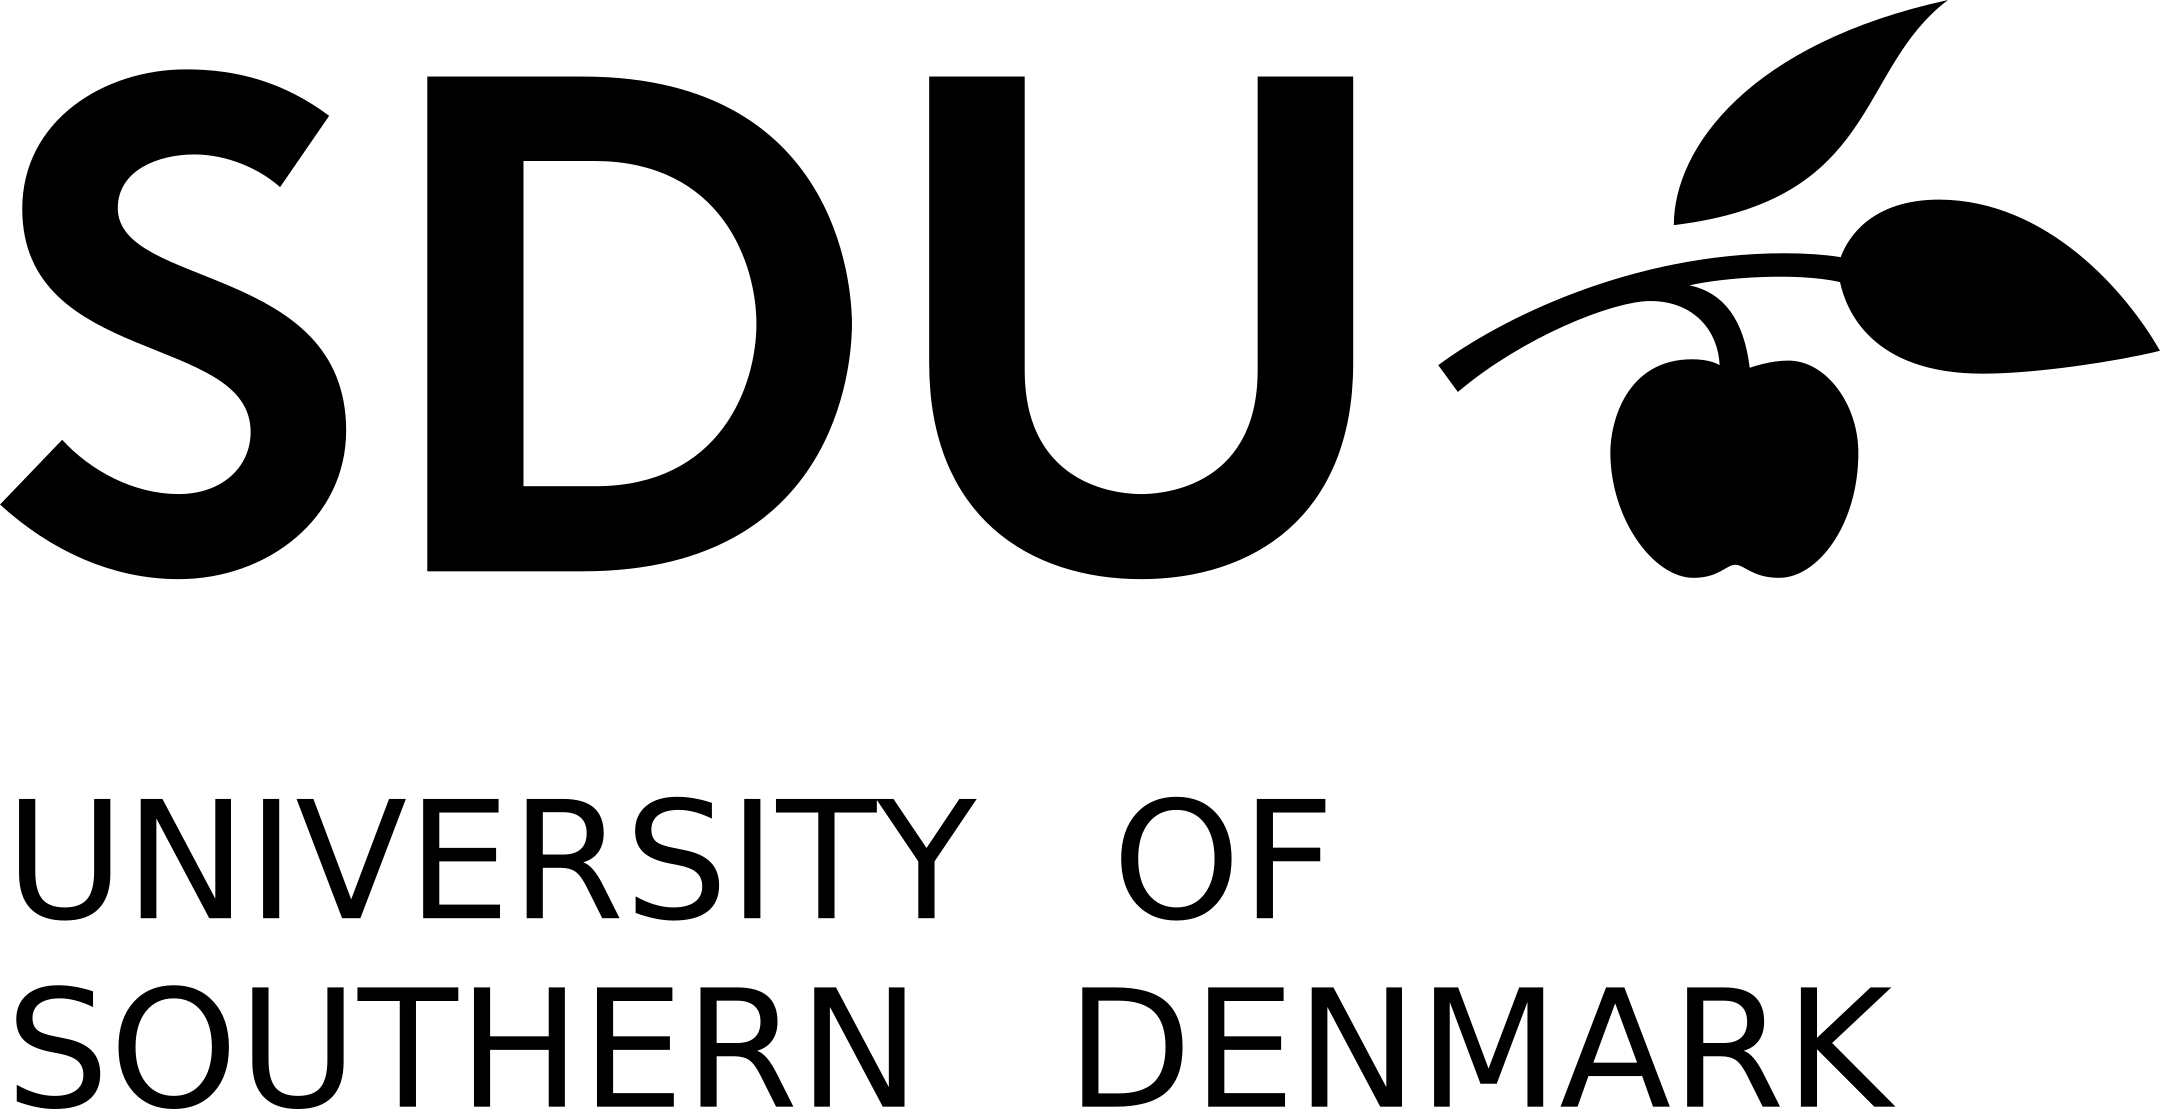
\includegraphics[scale=1]{SDU_logo}
    \vfill\
    \vspace{5mm}
    IMADA \\

    \textbf{\datedate}  \bf{at 10} \\[2\baselineskip]
\end{titlepage}

\renewcommand{\thepage}{\roman{page}}% Roman numerals for page counter
\tableofcontents
\newpage
\setcounter{page}{1}
\renewcommand{\thepage}{\arabic{page}}


\section{Introduction}

In the second project for DM818 we were tasked with making a particle simulator parallel, as a starting point we were given implementations in seriel, OpenMP, Pthreads, and MPI, The tasks were as follows, \\

\begin{itemize}
\item Optimize the serial ($ \theta = n^2$) to run in ($ \theta = n$) time
\item Implement a share memory implementation using Pthreads or Openmp
\item implement a distributed memory implementation using MPI
\end{itemize}

These different implementations should then be tested on the Edison Cluster at Nersc, Who has made computational time for the project. \\

\subsection{Work load and work distribution}
The project was done alone. 

\subsection{Issues}

The MPI code isn't functional, Therefor performance testing was also done using the code supplied from the lecturer. This code runs in $n^2$ time.

\newpage

\section{Design}

\subsection{Binning}
\begin{wrapfigure}{r}{0.25\textwidth} %this figure will be at the right
    \centering
    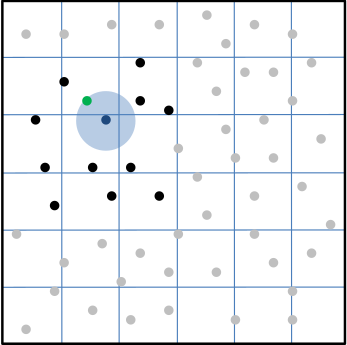
\includegraphics[width=0.25\textwidth]{grid.png}
\end{wrapfigure}
The binning algorithm was designed to make use of a grid, so it could work the same way of the matrix matrix blocking where it would interact with index +(-1,-1), to (1,1). \\

With a design like this elements can be dynamically removed and added which should remove the computational waste of clearing the grid and reinitializing it. it also allows the grid to be cleared on every cycle if it is needed. \\

\subsection{Serial with grid}
The serial gridded implementation is designed so it will only need itself and the 8 grids surrounding it to calculate the forces needed to move the particle.

\subsection{OPENMP with grid}
For designing the openmp implementation the gridded implementation was used as a starting point and the loops with apply force and move should be made parallel. the grid\_clear will have to have a barrier so threads won't start adding elements to the old grid that will be cleared by the main process. this will most likely cause some overhead.

\subsection{MPI with grid}

The reasoning behind a mpi implementation is to split the grid into smaller chunks, this can be done in a few different ways, the most apparent is splitting the chucks into smaller squares, but this requires the larger grid to be dividable by p, a different approach is to split the grid into rows. \\
For the sub cubed implementation we'll have to talk to the 8 surrounding threads which could induce a huge communication overhead, while the row wise implementation only required the threads to talk to 2 threads, and 1 for the top and lowest thread. \\

The communication per step would for each process be 2 x grid width x size of particle\_t. this is reasonable but at every step we'd need to sync so all threads have the required data. \\

\newpage

\section{Implementation}
\subsection{Grid}
The implementation of grid.cpp has a few small functions. the most important one being the get Neighbors functions. This returns the surrounding cells to the particle we wish to calculate the forces for. to The grid is stored as an array so to return the current cell we use the same calculation as we need with the blocked matrix matrix program
\begin{equation}
index = current location + row + column * row length
\end{equation}
The other functions of the grid that are of some important is the clear and add function. i also implemented a remove element since it was mentioned the other implementation could slow execution down, but as i was unable to get it to work i used the clear function.

\subsection{Serial grid}

The optimized serial implementation was modified by modifying the compute forces loops to work in a blocked manner. this was simply done by adding 2 for loops that go from index x-1 y-1 to x+1 y+1 and a inner loop the loops over all particles in those grids.\\
The move part of the code was modified by first clearing the grid as i was unable to get the computation to work currectly when just removing the element. and then calling the move function from common and adding the particle with its new values to the grid. 

\subsection{OPENMP grid}
The parallel area in the openmp implementation is all the code surrounding the main step for loop. Whats made parallel here is the apply force loop. this is done using \#pragma omp for, furthermore a \#pragma omp barrier is put in front of this here to make sure the master thread is done saving the data before other threads start using it. \\

The move loop is is made so only a single thread is doing this. when it was using multiple threads there was some issues with segmentation faults and instability. \\

\subsection{mpi grid}
The MPI with grid implementation was designed in so the grid would be split up into groups of rows, therefor each process would only have to communicate with 2 others in average case. This implementation meant that that at each step all processes would need to catch to to each other, this means that the implementation would have some overhead in the transfer stage, but it would be minimal as the average case all the cells have around the same amount of particles due to limits set in the base program. \\


\newpage
\section{Testing \& issues}

The different version's of the code have quite reasonable run times, and the accuracy of the code is good. however scaling on the parallel implementations isn't as good as it maybe should be.  \\

\subsection{MPI}
I wasn't able to get the MPI code to run in time for the deadline. I have included the code in the hand-in, but it doesn't run.

\section{Comparison}

\subsection{Serial}
The Old vs the new serial implementation provides the biggest boost in performance, this again proves the point from the previous assignment that the most important thing is to optimize your code before you start making it parallel. \\
\begin{wrapfigure}{r}{0.25\textwidth} %this figure will be at the right
    \centering
    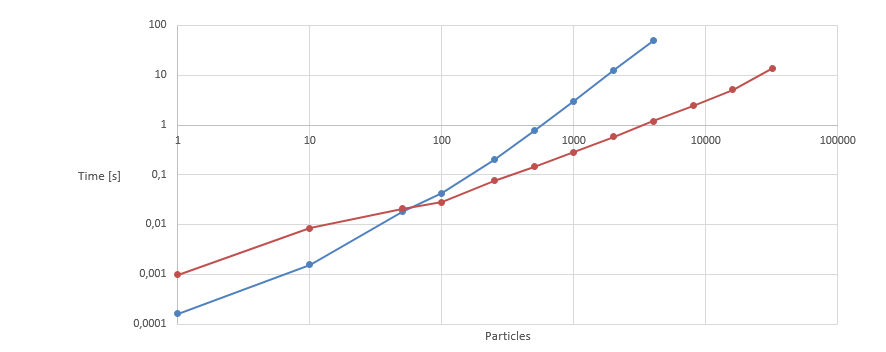
\includegraphics[width=0.45\textwidth]{oldvsnew}
\end{wrapfigure}

From looking on the graph it can be seen that the optimized version runs a lot faster than the old algorithm. this is confirmed by the auto grader which shows that the new algorithm runs in (n*1.048897) time.


\subsection{Openmp}
The OpenMP implementation provides a scaling efficiency of 0.48, which means there is a lot of overhead in this implementation. this is mostly due to some of the code being run in a single thread, and some barrier points where the different threads sync.

\section{Discussion}
The 3 different of the implementation differ from each other, OpenMP has it's good sides but it's limited to only 1 node, while MPI offers scaling across a huge cluster with many nodes. but it's also a lot more in dept to program, \\
They are designed for different use cases and it can clearly be seen which use cases they're for. \\
However it would say that the MPI implementation requires a lot more work, but it's also the only way to go for huge projects where one single machine can't run the entire problem at once. \\
This is also something that was mentioned in the beginning of the lecture, where it was said that "Parallel computing is a byproduct of the limitations of the thermodynamics of current computer hardware." \\
And it's entirely correct, we are limited by power consumption on CPU's, or rather heat dissipation. \\

\section{Conclusion}
Even though the entire project wasn't finished related to MPI, a lot was still learned and i gained some new tools to use for further projects. I'll keep improving my MPI programming and hopefully it'll be good enough for future use, i could see the course benefaction from smalling exercises resolved around MPI, so we can get a slight introduction to it, rather then getting thrown into the deep end, This is probably more of the concern from myself as I'm not a master or PHD student like some of the people taking the course.
\newpage
\section{appendix}
\subsection{data}
The whole excel sheet with data used for the graphs can be found here.
\begin{lstlisting}
https://1drv.ms/x/s!AjA16Is6byyvjvV-C5Vz5mWHLZhjig
\end{lstlisting}
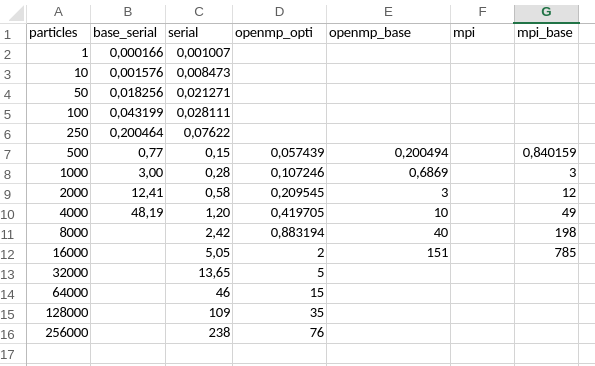
\includegraphics[scale=0.7]{alldata}

%\section{Code}
%\lstinputlisting{mandatory2/src/dgemm.cpp}

%\lstinputlisting{../src/test.cpp}

\end{document}

